\documentclass[tikz,margin=5mm]{standalone}
\usepackage{tikz}
\begin{document}
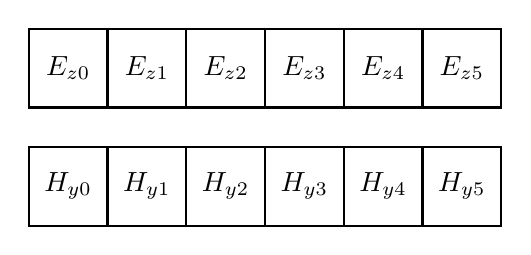
\begin{tikzpicture}
    \foreach \i/\val in {
        0/$E_{z\i}$,
	1/$E_{z\i}$,
	2/$E_{z\i}$,
	3/$E_{z\i}$,
        4/$E_{z\i}$,
	5/$E_{z\i}$,
  } {
    \draw[thick] (\i,1.5) rectangle ++(1,1);
    \node at (\i+0.5,2.0) {\val};
  }
    \foreach \i/\val in {
        0/$H_{y\i}$,
	1/$H_{y\i}$,
	2/$H_{y\i}$,
	3/$H_{y\i}$,
        4/$H_{y\i}$,
	5/$H_{y\i}$,
  } {
    \draw[thick] (\i,0) rectangle ++(1,1);
    \node at (\i+0.5,0.5) {\val};
  }
\end{tikzpicture}
\end{document}
